\section{Modelos de Distribución}
\subsection{Modelos discretos}
\begin{enumerate}[label=\color{red}\textbf{\Alph*)}, leftmargin=*]
	\item \lb{Uniforme discreta: $X\sim UD(n)$}
	\begin{itemize}[label=\color{red}\textbullet, leftmargin=*]
		\item \color{lightblue}Definición
	\end{itemize}
	Diremos que $X$ sigue una uniforme discreta de parámetro \lb{n}. Si toma exactamente \lb{$n$} valores, todos con la misma probabilidad.
	\begin{itemize}[label=\color{red}$-$]
		\item \lb{Rango o Soporte de $X$}
		
		$\sop(X)=(x_1,x_2,\dots,x_n)$
		\item \lb{Función puntual de probabilidad}
		
		$\begin{array}{l}
			p(x)=P(X=x)\\
			p(x_i)=\dfrac{1}{n}\;\forall x_i\in\sop(X)
		\end{array}$
		\item \lb{Esperanza o media de $X$}
		
		$E(X)=x_1\cdot\dfrac{1}{n}+x_2\cdot\dfrac{1}{n}+\cdots+x_n\cdot\dfrac{1}{n}=\dfrac{\displaystyle\sum_{i=1}^{n}x_i}{n}=\overline{x}$
		\item \lb{Varianza de $X$}
		
		$\begin{array}{l}
			\var(X)=\lbb{E(X^2)}{(\ast)}-(E(X))^2=\overline{x^2}-(\overline{x})^2=\sigma_x^2\\
			\lb{(\ast)}~E(x^2)=x_1^2\cdot\dfrac{1}{n}+x_2^2\cdot\dfrac{1}{n}+\cdots+x_n^2\cdot\dfrac{1}{n}=\dfrac{\sum x_i^2}{n}=\overline{x^2}
		\end{array}$
		
		\Ej\lb{:} $X=$"Resultado de lanzar un dado"$\sim UD(6)$
	\end{itemize}
	\item \lb{Modelo Bernoulli de parámetro $p,\:X\sim B(p)$}
	
	Llamaremos experimento Bernoulli de parámetro \lb{$p$} a un experimento aleatorio con sólo 2 resultados posibles que llamaremos \lb{éxito (E)} y \rc{fracaso (F)}. \begin{center}
		$\Omega=\{E,F\}$, con $p=P(E)=P(\text{"éxito"})$
	\end{center}
	\Ej
	
	Chequearemos una pieza al azar de una producción y miro si es defectuosa.
	\begin{itemize}[label=\color{red}\textbullet, leftmargin=*]
		\item \color{lightblue}Definición
	\end{itemize}
	A la \va $X=\begin{cases}
		1 & \text{si el experimento Bernoulli resultó éxito}\\
		0 & \text{en caso contrario}
	\end{cases}$
	
	$x:\Omega\longrightarrow\R$ se dice que sigue Bernoulli de parámetro \lb{$p$}, $X\sim B(p)$.
	\begin{itemize}[label=\color{red}$-$]
		\item \lb{Media o Esperanza de $X$}
		
		$E(X)=0\cdot(1-p)+1\cdot p=p$
		\item \lb{Varianza $X$}
		
		$\begin{array}{l}
			E(X^2)=0^2\cdot(1-p)+1^2\cdot p=p\\
			\var(X)=E(X^2)-(E(X))^2=p-p^2)p(1-p)=p\cdot q\text{ con }q=1-p
		\end{array}$
	\end{itemize}
	\Ej
	
	$X\equiv$ "Nº de piezas defectuosas al extraer al azar una de su producción".
	
	$X\sim B(p)$ donde $p=P$("Pieza defectuosa")$=$Tabla defectuosa en $m_i$ producción
	\item \lb{Modelo binomial de parámetro $n$ y $p, X\sim B(n,p)$}
	\begin{itemize}[label=\color{red}\textbullet, leftmargin=*]
		\item \color{lightblue}Definición
	\end{itemize}
	Consideremos un experimento Bernoulli de parámetro \lb{$p$}, y supongamos que se repite el experimento \lb{$n$} veces de formas independiente.
	
	La \va $X=$"Nº de éxitos obtenidos en las \lb{$n$} repeticiones del experimento" sigue un modelo Binomial, $X\sim B(n,p)$
	\begin{itemize}[label=\color{red}$-$, leftmargin=*]
		\item \lb{Soporte o rango $X$}
		
		$\sop(X)=\{0,1,\dots,n\}$
		\item \lb{Función puntual de probabilidad}
		
		$\begin{array}{l}
			p(x)=P(X=x)\\
			p(0)=P(X=0)=P(F_1\cap F_2\cap\dots\cap F_n)=\lb{\left\{\begin{tabular}{l}
					linealmente\\
					independiente
				\end{tabular}\right\}}=\prod_{i=1}^{n}P(F_1)\\
			p(1)=P(X=1)=P(E_1\cap F_2\cap\dots\cap F_n)\cup\dots\cup P(F_1\cap F_2\cap\dots\cap E_n)=np(1-p)^{n-1}=npq^{n-1}\\
			p(2)=P(X=2)=\binom{n}{2}\cdot p^2\cdot(1-p)^{n-2}\\
			p(x)=P(X=x)=\binom{n}{x}\cdot p^x\cdot(1-p)^{n-x}\quad\forall x\in\{0,1,2,\dots,n\}
		\end{array}$
		\begin{itemize}[label=\color{red}\textbullet, leftmargin=*]
			\item \color{lightblue}Observación
		\end{itemize}
		El modelo $B(n,p)$ se obtiene como suma de \lb{$n$} modelos Bernoulli de parámetro \lb{$p$ independientes}.
		
		$\begin{array}{l}
			X_i\sim B(p),\; i=1,\dots,n\:\lb{\text{independientes}}\\
			X=X_1+X_2+\cdots+X_n\sim B(n,p)\\
			E(X)=E(X_1)+E(X_2)+\cdots+E(X_n)=n\cdot p
		\end{array}$
		\item \lb{Varianza de $X\sim B(n,p)$}
		
		$\var(X)=\var(X_1+\cdots+X_n)=\var(X_1)+\var(X_2)+\cdots+\var(X_n)=n\cdot p\cdot(1-p)=npq$
		
		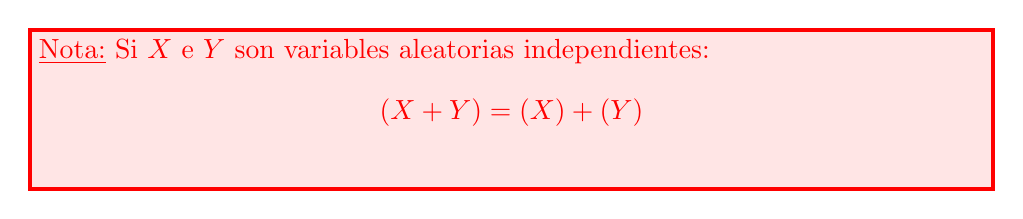
\begin{tikzpicture}
			\node[red, draw=red, fill=red!10, line width=1.5, text width=12cm] {\underline{Nota:} Si $X$ e $Y$ son variables aleatorias independientes: \[ \var(X+Y)=\var(X)+\var(Y) \]};
		\end{tikzpicture}
		\begin{itemize}[label=\color{red}\textbullet, leftmargin=*]
			\item \lb{Propiedad:} la binomial es reproductora respecto al parámetro \lb{$n$}. Es decir:
			\begin{itemize}[label=$-$]
				\item Si $X\sim B(n_1,p),Y\sim B(n_2,P)$ independientes, entonces $X+Y\sim B(n_1+n_2,p)$
			\end{itemize}
		\end{itemize}
	\end{itemize}
	\bu{Ejemplo 1}
	
	Consideremos una urna con 20 bolas, de las cuales 8 son blancas y 12 son negras. Extremos 5 bolas una a una \lb{con reemplazamiento}.
	
	La \va $X\equiv$"Nº de bolas blancas en la muestra de tamaño 5"$\sim B\left(n=5,p=\dfrac{8}{20}=\dfrac{2}{5}\right)$
	
	\bu{Ejemplo 2}
	
	Sabemos que la tasa de defectuosas de una linea productiva es del 7\%. Suponemos producción muy elevada y empaqueto las piezas en cajas de 15 unidades. 
	
	$X\equiv$"Nº de piezas defectuosas en una caja de 15 unidades"$\sim B(n=15,p=0.07)$
	
	
\begin{tikzpicture}
		\node[red, draw=red, fill=red!10, line width=1.5] {\underline{Nota:} Disponemos de tablas para calcular las probabilidades puntuales};
	\end{tikzpicture}
	\item \lb{Modelo hipergeométrico, $X\sim M(N,a,n)$}
	
	Es como la Binomial pero los experimentos Bernoullis no se realizan de forma independiente. Por ejemplo, si se realizan extracciones \lb{sin reemplazamiento}.
	
	$\bboxed{\begin{array}{l}
			\lb{N\longrightarrow}\text{ nº de elementos de población}\\
			\lb{a\longrightarrow}\text{ nº de éxitos de la población}\\
			\lb{n\longrightarrow} \text{ tamaño de la muestra extraída}\\
			\lb{n=N-a\longrightarrow}\text{ nº de fracasos posibles}
	\end{array}}$

La \va $X\equiv$"Nº de éxitos en la muestra de tamaño $n$"$\sim+(N,a,n)$

$\begin{array}{l}
	\sop(X)=\{\lbb{\max(0,N-b)}{},\dots,\min(n,a)\}\\
	\lb{P(X=x)=P(\underbrace{E\cap E\cap \dots\cap E}_x\cap\underbrace{F\cap F\cap\dots\cap F}_{n-x})=\dfrac{\dbinom{a}{x}\cdot\dbinom{N-a}{n-x}}{\dbinom{N}{n}}=\dfrac{\dbinom{a}{x}\cdot\dbinom{b}{n-x}}{\dbinom{a+b}{n}}}\\
	\lb{E(X)=n\cdot \dfrac{a}{N}}\\
	\lb{\var(X)=n\cdot\dfrac{a}{N}\cdot\left(\dfrac{N-a}{N}\right)\cdot\left(\dfrac{N-n}{N-1}\right)}
\end{array}$

\begin{tikzpicture}
	\node[red, draw=red, fill=red!10, line width=1.5, text width=\textwidth] {\underline{Nota:} Si $\dfrac{n}{N}\le0.10$, entonces podemos aproximar la $H(N,a,n)$ por una \[ B\left(n,p=\dfrac{a}{N}\right) \]En este caso, el muestreo sin reemplazamiento sería equivalente al muestreo sobre \underline{poblaciones infinitas}.};
\end{tikzpicture}

\Ej

Una urna con 20 bolas de las cuales son 8 blancas y 12 negras. Se extrae una muestra de tamaño 5 \lb{sin reemplazamiento}.
\begin{center}
	$X\sim$"Nº de bolas blancas en la muestra"$\sim H(N=20,a=8,n=5)$
\end{center}
\item \lb{Geométrica, $X\sim G(p)$}

Consideramos experimento Bernoulli$(p)$ que se realiza de forma independiente hasta obtener el $1^{\mathrm{er}}$ éxito.\\
La \va $X\equiv$"Nº de fracasos hasta obtener el $1^{\mathrm{er}}$ éxito"$\sim G(p)$.\\
$\sop(X)=\{0,1,2,\dots\}=\N$\\
$P(X=x)=P(\lbb{F_1\cap F_2\cap \dots\cap F_x}{x~\mathrm{fracasos}}\cap\lbb{E_1}{\text{éxito}})=(1-p)^x\cdot p=p\cdot q^x$\\
$E(X)=\sum_{x=0}^{\infty}x\cdot p\cdot q^x=\sum_{x=1}^{\infty}xpq^x=pq\sum_{x=1}^{\infty}xq^{x-1}=pq\sum_{x=1}^{\infty}\dfrac{\partial}{\partial q}(q^x)=pq\dfrac{\partial}{\partial q}\lbb{\left(\sum_{x=1}^{\infty}q^x\right)}{\dfrac{q}{1-q}}=pq\dfrac{\partial}{\partial q}\left(\dfrac{q}{1-q}\right)=pq\dfrac{1-q+q}{(1-q)^2}=\dfrac{\cancel{p}q}{p^{\cancel{2}}}=\bboxed{\dfrac{q}{p}=E(X)}$

Tenemos la suma infinita de una progresión geométrica de razón $q_\infty\in(0,1)$, por tanto converge.

\fcolorbox{red}{red!10}{\rc{\underline{Nota:} $\sum_{i=1}^{\infty}a_i=\dfrac{a_1}{1-r},\:a_n=a_1\cdot r^{n-1}$ si $|r|<1$}}

$\var(X)=E(X^2)-(E(X))^2=\dfrac{2q^2}{p^2}+\dfrac{p}{q}-\left(\dfrac{q}{p}\right)^2=\dfrac{2q^2+pq-q^2}{p^2}=\dfrac{q\overbrace{(q+p)}^1}{p^2}=\bboxed{\dfrac{q}{p^2}}$

Vamos a calcular $E(X(X-1))=E(X^2)-E(X)\longrightarrow E(X^2)=E(X(X-1))+E(X)=\dfrac{2q^2}{p^2}+\dfrac{q}{p}$

{\color{lightblue}
$E(X(X-1))=\sum_{x=0}^{\infty}x(x-1)\cdot p\cdot q^x=\sum_{x=2}^{\infty}x(x-1)pq^x=pq^2\sum_{x=2}^{\infty}x(x-1)q^{x-2}=pq^2\sum_{x=2}^{\infty}\dfrac{\partial^2}{\partial q^2}(q^x)=pq^2\dfrac{\partial^2}{\partial q^2}\underbrace{\left(\sum_{x=2}^{\infty}q^x\right)}_{\dfrac{q^2}{1-q}}=pq^2\dfrac{\partial^2}{\partial q^2}\left(\dfrac{q^2}{1-q}\right)=(\ast)$\\
$\dfrac{\partial}{\partial q}\left(\dfrac{q^2}{1-q}\right)=\dfrac{2q(1-q)+q^2}{(1-q)^2}=\dfrac{2q-q^2}{(1-q)^2}\longrightarrow\dfrac{\partial^2}{\partial q^2}\left(\dfrac{q^2}{1-q}\right)=\dfrac{(2-2q)(1-q)^2+2(2q-q^2)(1-q)}{(1-q)^4}=\dfrac{2\cancel{(1-q)}\overbrace{\left((1-q)^2+(2q-q^2)\right)}^{1-\cancel{2q}+\cancel{q^2}+\cancel{2q}-\cancel{q^2}}}{(1-q)^{\cancel{4}}}=\dfrac{2}{(1-q)^3}=\dfrac{2}{p^3}$\\
$(\ast)=\cancel{p}q^2\dfrac{2}{p^{\cancel{3}}}=\dfrac{2q^2}{p^2}$
}
\item \lb{Binomial negativa, $X\sim BN(n,p)$}

Consideramos experimento Bernoulli$(p)$ y realizamos el experimento de forma independiente hasta obtener el $n$-ésimo éxito.\\
La \va $X\equiv$"Nº de fracasos hasta obtener el \lb{$n$-ésimo} éxito" $X\sim BN(n,p)$
\begin{itemize}
	\item $\sop(X)=\{0,1,2,\dots\}=\N$
	\item $P(X=x)=P\lbb{(E\cap P\cap\dots\cap\bboxed{E})}{n+x\text{ posiciones}}=\bboxed{\dbinom{n+x-1}{x}\cdot(1-p)^x\cdot p^n}$
\end{itemize}
$\begin{aligned}
	\text{Sea }y_1&=\text{"Nº de fracasos hasta $1^{\mathrm{er}}$ éxito"}\sim G(p)
	y_2&=\text{"Nº de fracasos hasta $1^{\mathrm{er}}$ y $2^{\mathrm{er}}$ éxito"}\sim G(p)\\
	&\vdots\\
	y_n&=\text{"Nº de fracasos entre $(n-1)$-ésimo y $n$-ésimo éxito"}\sim G(p)
\end{aligned}$

$x=y_1+y_2+\cdots+y_n$ con $y_j$ independiente $\forall j=1,2,\dots,n$\\
$E(X)=E(y_1)+\cdots+E(y_n)=\dfrac{q}{p}+\dfrac{q}{p}+\cdots+\dfrac{q}{p}=\bboxed{\dfrac{nq}{p}}$\\
$\var(X)=\var(y_1)+\cdots+\var(y_n)=\bboxed{\dfrac{nq}{p^2}}$

\begin{tikzpicture}
	\node[red, draw=red, fill=red!10, line width=1.5, text width=\textwidth] {\underline{Nota 1:}\\
	$X=$"Nº de fracasos hasta obtener $1^{\mathrm{er}}$ éxito"$\sim G(p)$\\
	$Y=$"Nº de experimentos necesarios para obtener $1^{\mathrm{er}}$ éxito"\\
	$Y=X+1\cdot E(Y)=E(X)+1=\dfrac{q}{p}+1=\boxed{\dfrac{1}{p}}$\[ \var(Y)=\var(X)=\boxed{\dfrac{q}{p^2}} \]
	};
\end{tikzpicture}

$P(Y=3)=P(X=2)$

\begin{tikzpicture}
	\node[red, draw=red, fill=red!10, line width=1.5, text width=\textwidth] {\underline{Nota 1:}\\
		$X=$"Nº de fracasos hasta obtener $n$-ésimo éxito"$\sim G(p)$\\
		$Y=$"Nº de experimentos necesarios para obtener el $n$-ésimo éxito"\\
		$Y=X+n\cdot E(Y)=E(X)+n=\dfrac{q}{p}+n=n\cdot\left(\dfrac{q}{p}+1\right)=\boxed{\dfrac{n}{p}}$\[ \var(Y)=\var(X)=\boxed{\dfrac{nq}{p^2}} \]
	};
\end{tikzpicture}
\item \lb{Modelo de Poisson, $X\sim P(\lambda)$}
\begin{itemize}[label=\color{red}\textbullet, leftmargin=*]
	\item \color{lightblue}Definición
\end{itemize}
Diremos que la \va $X$ sigue un modelo de Poisson, $X\sim P(\lambda)$, de parámetro $\lambda$ si su \fpp es:\[ p(x)=P(X=x)=e^{-1}\cdot\dfrac{\lambda^x}{x!},\:x=1,2,\dots,\N \]Probamos que $E(X)=\lambda$ y $\var(X)=\lambda$.\\
¿Qué fenómenos modeliza la Poisson?
\begin{enumerate}[label=\color{lightblue}\underline{Escenario \arabic*:}]
	\item Cuando tengamos una Binomial, $B(n,p)$, con \lb{$n$} grande y \lb{$p$} pequeña.
	\begin{itemize}[label=\color{red}$-$, leftmargin=*]
		\item \lb{Regla:} $n\ge20,p\le0.1,n\cdot p\le5\longrightarrow$ aproximación $B(n,p)$ por $P(\lambda=np)$.
	\end{itemize}
	\item Contar el número de veces que ocurre un suceso sobre un soporte continuo (intervalo de tiempo/superficie).
	\begin{multicols}{2}
		$E(X)=\lambda$\\
		\fcolorbox{red}{red!10}{\rc{\underline{Nota:} $e^a=\sum_{n=0}^{\infty}\dfrac{a^n}{n!}$}}
	\end{multicols}
	$E(X)=\sum_{x=0}^{\infty}=x\cdot e^{-\lambda}\cdot\dfrac{\lambda^x}{x!}=\sum_{x=1}^{\lambda}xe^{-1}\cdot\dfrac{\lambda^x}{x!}=e^{-\lambda}\cdot\lambda\sum_{x=1}^{\infty}\dfrac{\lambda^{x-1}}{(x-1)!}=e^{-\lambda}\cdot\lambda\sum_{n=0}^{\infty}\dfrac{\lambda^n}{n!}=e^{-\lambda}\cdot\lambda\cdot e^{\lambda}=\bboxed{\lambda}$\\
	$\begin{array}{l}
		\var(X)=E(X^2)-(E(X))^2\\
		E(X^2)=E(X(X-1))+E(X)\\
		X(X-1)=X^2-X\\
		x^2=X(X-1)+X\\
	\end{array}$\\
	$E(X(X-1))\sum_{x=0}^{\infty}x(x-1)\cdot e^{-\lambda}\cdot\dfrac{\lambda^x}{x!}=e^{-\lambda}\cdot\lambda^2\sum_{x=0}^{\infty}x(x-1)\cdot\dfrac{\lambda^{x-2}}{(x-2)!}=e^{-\lambda}\cdot\lambda^2\cdot\sum_{n=0}^{\infty}\dfrac{\lambda^n}{n!}=\underbrace{e^{-\lambda}\cdot e^{\lambda}}_1\cdot\lambda^2=\bboxed{\lambda^2}$\\
	$\bboxed{\var(X)=\lambda^2+\lambda-\lambda^2=\lambda}$
\end{enumerate}
\begin{itemize}[label=\color{red}\textbullet, leftmargin=*]
	\item \color{lightblue}Propiedades
\end{itemize}
Si $X_1\sim P(\lambda_1)$ y $X_2\sim P(\lambda_2)$ independientes $\longrightarrow X_1+X_2\sim P(\lambda_1+\lambda_2)$. La Poisson es reproductiva. 
\end{enumerate}
\subsection{Modelos continuos}
\begin{enumerate}[label=\textbf{\color{red}\Alph*)}, leftmargin=*]
	\item \lb{Uniforme, $\sim U(a,b)$}
	\begin{itemize}[label=\color{red}\textbullet, leftmargin=*]
		\item \color{lightblue}Definición
	\end{itemize}
	Diremos que $X$ sigue una distribución uniforme en el intervalo $(a,b)$ si tiene función de densidad constante\begin{center}
		$f(x)=\begin{cases}
			\dfrac{1}{b-a} & \text{si }x\in(a,b)\\
			0 & \text{si }x\notin(a,b)
		\end{cases}$\qquad\begin{tikzpicture}[baseline=(current bounding box.center)]
		\fill[fill=lightblue!10] (1,1) rectangle (2,0);
		\draw (-1,0) -- (5,0);
		\draw (0,-1) -- (0,2) node[above] {$f(x)$};
		\draw[lightblue, line width=2] (-1,0) -- (1,0) node[below] {$a$};
		\draw[lightblue, line width=2] (1,1) -- (3,1);
		\draw[lightblue, line width=2] (3,0) node[below] {$b$} -- (5,0);
		\foreach \x in {0.2,4.2}{
		\draw[blue] (\x,0.1) -- (\x,-0.1) node[below] {$x$};
		}
		\draw[blue] (2,1) -- (2,0) node[below] {$x$};
		\draw[lightblue, dashed] (1,0) -- (1,1);
		\draw[lightblue, dashed] (3,0) -- (3,1);
		\draw[lightblue] (0.1,1) -- (-0.1,1) node[left] {$\dfrac{1}{b-a}$};
		\end{tikzpicture}
	\end{center}
	La función de distribución vale:
	
	$\begin{array}{l}
		F(x)=\int_{-\infty}^{x}f(t)\dt\\
		F(x)=\begin{cases}
			0 & \text{si }x\le a\\
			\dfrac{x-a}{b-a} & \text{si }a\le x\le b\\
			1 & \text{si }x\ge b
		\end{cases}\\
		\var(X)=E(X^2)-(E(X))^2=\lb{(\ast)}\\
		E(X)=\int_{-\infty}^{+\infty}xf(x)\dx=\int_{a}^bx\cdot\dfrac{1}{b-a}\dx=\dfrac{1}{b-a}\left[\dfrac{x^2}{2}\right]_a^b=\dfrac{b^2-a^2}{2(b-a)}=\dfrac{\cancel{(b-a)}(b+a)}{2\cancel{(b-a)}}=\bboxed{\dfrac{b+a}{2}}\\
		E(X^2)=\int_a^bx^2\cdot\dfrac{1}{b-a}\dx=\dfrac{1}{b-a}\left[\dfrac{x^3}{3}\right]_a^b=\dfrac{b^3-a^3}{3(b-a)}=\dfrac{\cancel{(b-a)}(b^2+ab+a^2)}{3\cancel{(b-a)}}=\bboxed{\dfrac{b^2+ab+a^2}{3}}\\
		\lb{(\ast)=}\dfrac{b+a}{2}-\dfrac{b^2+ab+a^2}{3}=\dfrac{3(b+a)-2(b^2-2ab-2a^2)}{6}=\bboxed{\dfrac{-2b^2-2a^2+3b-2ab+3a}{6}}
	\end{array}$
	
	\Ej
	
	$X=$"Seleccionar al azar un número en el intervalo $(0,1)$"
	
	\begin{tikzpicture}
		\draw (-1,0) -- (3,0);
		\draw (0,-0.5) -- (0,1.5) node[above] {$F(x)\to X\sim U(0,1)$};
		\draw[lightblue, line width=2] (-1,0) -- (1,0) node[below] {$a$} -- (2,1) -- (3,1);
		\draw[lightblue, dashed] (2,1) -- (2,0) node[below] {$b$};
		\draw[lightblue] (0.1,1) -- (-0.1, 1) node[left] {$1$};
	\end{tikzpicture}
	\item \lb{Exponencial, $X\sim\mathrm{Exp}(\lambda)$}
	\begin{itemize}[label=\color{red}\textbullet, leftmargin=*]
		\item \color{lightblue}Definición
	\end{itemize}
	Diremos que $X$ sigue $\mathrm{Exp}(\lambda)$ si su densidad es: \[ f(x)=\begin{cases}
		\lambda e^{-\lambda x} & \text{si }x\ge0 \text{ con }\lambda>0\\
		0 & \text{en el resto}
	\end{cases} \]
	
		\begin{tikzpicture}[scale=1.5]
			\fill[fill=lightblue!10, domain=0:1, samples=100] plot (\x, {exp(-0.5*\x)}) -- (1,0) -- (0,0) -- cycle;
			\draw (-1.5,0) -- (3,0) ;
			\draw (0,-0.5) -- (0,1.5) node[above] {$F(x)$};
			\draw[lightblue, domain=0:3, samples=100, line width=2] plot (\x, {exp(-0.5*\x)});
			\draw[lightblue, line width=2] (-1.5,0) -- (0,0);
			\draw[blue] (-1,0.1) -- (-1,-0.1) node[below] {$x$};
			\draw[blue] (1,0) node[below] {$x$} -- (1,{exp(-0.5*1)});
			\node[lightblue, left] at (0,1) {$\lambda$};
		\end{tikzpicture}
		
		La función de distribución:\[ F(x)=\int_{-\infty}^{x}f(t)\dt \]
		\begin{itemize}
			\item Si $x\ge0\longrightarrow F(x)=\int_0^x\lambda e^{-\lambda t}\dt=\left[-e^{-\lambda t}\right]_0^x=-e^{-\lambda x}+1=\bboxed{1-e^{-\lambda x}}$\[ F(x)=\begin{cases}
				0 & \text{si }x\le 0\\
				1-e^{-\lambda x} & \text{si }x\ge0
			\end{cases} \]
			\item $E(X)=\int_{-\infty}^{+\infty}xf(x)\dx=\int_{0}^{+\infty}x\lambda e^{-\lambda x}\dx=\lambda\int_{0}^{+\infty}xe^{-\lambda x}\dx=\left\{\begin{array}{ll}
				x=u & \dx=\du\\
				e^{-\lambda x}\dx=\dv & v=-\dfrac{1}{\lambda}e^{-\lambda x}
			\end{array}\right\}=\lambda\cdot\left(\left[x\cdot\dfrac{1}{\lambda}e^{-\lambda x}\right]_0^{+\infty}-\int_0^{+\infty}-\dfrac{1}{\lambda}e^{-\lambda x}\dx\right)=\lambda\cdot\left(-\dfrac{1}{\lambda}\right)\cdot\left(0-\left[\dfrac{1}{\lambda}e^{-\lambda x}\right]_0^{+\infty}\right)=\bboxed{\dfrac{1}{\lambda}}$
			
			$\lim_{x\to+\infty}xe^{-\lambda x}=\lim_{x\to+\infty}\dfrac{x}{e^{\lambda x}}=\dfrac{\infty}{\infty}=\left\{\text{L'Hôpital}\right\}=\lim_{x\to+\infty}\dfrac{1}{\lambda e^{\lambda x}}=\dfrac{1}{\infty}=0$
			
			$\begin{cases}
				\Gamma(p)=\int_{0}^{+\infty}t^{p-1}\cdot e^{-t}\dt\\
				\Gamma(n)=(n-1)!
			\end{cases}$
			\item $\var(X)=E(X^2)-(E(X))^2=\lb{(\ast)}$
			
			$E(X^2)=\int_{0}^{+\infty}x^2\cdot \lambda e^{-\lambda x}\dx=\left\{\begin{array}{l}
				t=\lambda x\\
				x=\dfrac{t}{\lambda}\longrightarrow\dx=\dfrac{1}{\lambda}\dt
			\end{array}\right\}=\lambda\cdot\int_{0}^{+\infty}\dfrac{t^2}{\lambda^2}e^{-t}\cdot\dfrac{1}{\lambda}\dt=\dfrac{1}{\lambda^2}\int_{0}^{+\infty}t^2\cdot e^{-t}\dt=\bboxed{\dfrac{2}{\lambda^2}}$\\
			$\lb{(\ast)=}\dfrac{2}{\lambda^2}-\left(\dfrac{1}{\lambda}\right)^2=\bboxed{\dfrac{1}{\lambda^2}}$
			\item ¿Moda? El máxumo de $f(x)$ se alcanza en $x=0=$ Moda.
			\item Mediana: $Me=$punto que cumple $F(Me)=\dfrac{1}{2}=1-e^{-\lambda x}\longrightarrow e^{-\lambda x}=\dfrac{1}{2}\longrightarrow\dfrac{1}{e^{\lambda x}}=\dfrac{1}{2}\longrightarrow e^{\lambda x}=2\longrightarrow\lambda x=\ln(2)\longrightarrow\bboxed{x=\dfrac{1}{\lambda}\cdot\ln(2)}$
		\end{itemize}
		\begin{itemize}[label=\color{red}\textbullet, leftmargin=*]
			\item \color{lightblue}Propiedad (falta de memoria)
		\end{itemize}
		Si $X\sim\mathrm{Exp}(\lambda)$, entonces $P(X>t+x/X>t)=P(X>x)$
		\begin{itemize}[label=\color{red}\textbullet, leftmargin=*]
			\item \color{lightblue}Demostración
		\end{itemize}
		$P(X>t+x/X>t)=\dfrac{P\left((X>t)\cap(X>t+x)\right)}{P(X>t)}=\dfrac{P(X>t+x)}{P(X>t)}=\dfrac{e^{-\lambda(t+x)}}{e^{-\lambda t}}=e^{-\lambda x}=P(X>x)$
		
		\begin{center}
			\begin{tikzpicture}
				\draw (-1,0) -- (3,0);
				\draw[lightblue, [-latex] (0,1) -- (3,1);
				\draw[blue, [-latex] (1,0.5) -- (3,0.5);
				\draw (0,0.1) -- (0,-0.1) node[below] {$x$};
				\draw (1,0.1) -- (1,-0.1) node[below] {$t+x$};
			\end{tikzpicture}
		\end{center}
		\Ej
		
		"Tiempo de vida de un dispositivo que no envejece"
		\item \lb{Weibull, $X\sim W(a,b)$}
		
		Si $Y\sim\mathrm{Exp}(\lambda)\longrightarrow x=Y^c$ es una Weibull $c>0,c=\dfrac{1}{a}\quad\lambda=b^{-a}$
		\begin{itemize}
			\item Si $c=1$ sale la exponencial
			\item Sirve para modelizar tiempo de vida con tasas de fallo decreciente, constante o creciente.
		\end{itemize}
		$X=$"Tiempo de vida de un dispositivo"
		\item \lb{Gamma, $X\sim\mathrm{Gamma}(a,b)$}
		\begin{itemize}
			\item Es una generalización Exponencial.
			\item Para $a=1$ se obtiene $\mathrm{Exp}(\lambda =b)$
			\item Si $a\le n$ entero positivo, se denomina distribución Erlang \lb{$(\mathrm{Gamma}(\mathrm{int}(a),b))$}, que es suma de exponenciales independientes.
		\end{itemize}
		$X=$"Tiempo trascurrido hasta el $n$-ésimo suceso o evento"
		\item \lb{Modelo Normal, $X\sim N(\mu,\sigma)$}
		\begin{itemize}[label=\color{red}\textbullet, leftmargin=*]
			\item \color{lightblue}Definición
		\end{itemize}
		Diremos que $X$ sigue una $N(\mu,\sigma)$ si su densidad es: \[ f(x)=\dfrac{1}{\sigma\sqrt{2\pi}}e^{-\frac{(x-\mu)^2}{2\sigma^2}}\:\forall x\in\R \]
		\begin{enumerate}[label=\color{red}\alph*)]
			\item \lb{¿Cómo es la densidad?}
			
			\begin{minipage}[l]{0.4\textwidth}
				\begin{tikzpicture}
					\begin{axis}[
						ymin=-0.1,
						domain=-3:3,
						samples=100,
						axis lines=middle,
						legend pos=north east,
						xtick=\empty, ytick=\empty,
						]
						\addplot[lightblue, mark=none] {1/(1*sqrt(2*pi)) * exp(-((x - 0)^2)/(2*1^2))};
						\node[below] at (axis cs:-1.5,0) {$\mu-\sigma$};
						\node[below] at (axis cs:1.5,0) {$\mu+\sigma$};
					\end{axis}
				\end{tikzpicture}
			\end{minipage}\quad\begin{minipage}[r]{0.5\textwidth}
			\begin{itemize}
				\item Es simétrica con eje de simétrica $x=\mu$.
				\item En $x=\mu$ tiene un máximo se puede ver que $f'(x=\mu)=0$ y $f''(x=\mu)<0$.
				\item Tiene puntos de inflexión en $x=\mu-\sigma$ y $x=\mu+\sigma$. Comprobar que $f'''(x)=0\longleftrightarrow x=\mu\pm\sigma$
				\item Tiene asíntota horizontal $y=0$
			\end{itemize}
			\[ \lim_{x\to-\infty}f(x)=\lim_{x\to+\infty}f(x)=0 \]
			\end{minipage}
			
			\begin{tikzpicture}
				\node[ draw=lightblue, fill=lightblue!10, line width=1.5, text width=12cm] {Se puede demostrar:\\
				\begin{enumerate}[label=\color{lightblue}\arabic*)]
					\item Que $f(x)$ es densidad
					\item Que $E(x)=\mu$
					\item Que $\sigma(X)=\sigma,\:\var(X)=\sigma^2$
					\end{enumerate}};
			\end{tikzpicture}
			\item \lb{¿Cuándo se usa la Normal?}
			\begin{itemize}
				\item Para modelizar errores de medición
				\item Para aproximar la Binomial y Poisson
				\item Para Inferencia (Teorema Central del Límite)
			\end{itemize}
			\item \lb{Función distribución}
			\begin{itemize}
				\item No existe la primitiva de $f(x)$
				\item Se obtiene mediante integración numérica
				
				Tenemos tabulada la $N(\mu=0,\sigma=1)$
			\end{itemize}
			\item \lb{Tipificar:} Si $X\sim N(\mu,\sigma)\longrightarrow z=\dfrac{X-\mu}{\sigma}\sim N(0,1)$
			
			Entonces podremos calcular la probabilidad de la $N(\mu,\sigma)$ a partir de la tabla $N(0,1)$ si tipificamos.
			\item \lb{Propiedades de la Normal}
			\begin{enumerate}[label=\color{lightblue}\arabic*)]
				\item Si $X\sim N(\mu_X,\sigma_X)\longrightarrow Y=\underset{a,b\in\R}{aX+b}\sim N(\mu_Y=a\mu_X+b,\sigma_Y=|a|\cdot\sigma_X)$
				\item Si $X_1,X_2,\dots,X_n$ sea $N(\mu_i,\sigma_i)\;i=1,2,\dots,n$, independientes entocnes $Y=X_1+X_2+\cdots+X_n\sim N(\mu_Y=\mu_1+\cdots+\sigma_n,\sigma_Y=\sqrt{\sigma_1^2+\cdots+\sigma_n^2})$
				\item \begin{itemize}
					\item Si $X\sim B(n,p)$ con $n$ grande $(n\ge30)$ y $np(1-p)>5$, entonces $X$ se puede aproximar por $Y\sim N(\mu=np,\sigma=\sqrt{np(1-p)})$
					\item Si $X\sim P(\lambda)$ como $\lambda\ge5$, entonces $X$ se puede aproximar por $Y\sim N(\mu=\lambda,\sigma=\sqrt{\lambda})$. La aproximación se puede mejorar realizando corrección por continuidad \[ P(X=a)\simeq P(a-0.5\le Y\le a+0.5) \]
					
				\end{itemize}
			\end{enumerate}
		\end{enumerate}
\end{enumerate}
\begin{minipage}[l]{0.3\textwidth}
	\begin{tikzpicture}
		\draw (-0.5,0) -- (2.5,0);
		\draw (-0.5,2) -- (2.5,2);
		\draw[lightblue, line width=1.5] (0,0) node[below] {97.5}-- (0.5,2) -- (1,0) node[below] {98.5} -- (1.5,2) -- (2,0) node[below] {99.5} -- (2.5,2);
		\foreach \x in {0,1,2}{
		\fill[lightblue] (\x,0) circle (2pt);
		\fill[lightblue] ({\x+0.5},2) circle (2pt);
		}
	\end{tikzpicture}
\end{minipage}\qquad$\begin{array}{l}
B(n=100,p=0.1)\\
B(n,p)\\
P(17<X\le35)\simeq P(17.5\le X\le 35.5)\\
N(\mu=np=10,\sigma=3)
\end{array}$

$P(X>20)\simeq P(X\ge20.5)$

\begin{tikzpicture}
	\begin{axis}[
		ymin=-0.1,
		xmax=3.2,
		domain=-3:3,
		samples=100,
		axis lines=middle,
		legend pos=north east,
		xtick=\empty, ytick=\empty,
		width=10cm,
		]
		\addplot[lightblue, mark=none] {1/(1*sqrt(2*pi)) * exp(-((x - 0)^2)/(2*1^2))};
		\node[below] at (axis cs:2.9,0) {100};
		\node[below] at (axis cs:2.5,0) {99};
		\node[below] at (axis cs:2,0) {98};
	\end{axis}
\end{tikzpicture}